\chapter{Sound, Oscillators, and the Deferred Second Law}

These notes follow Leonard Susskind's seventh lecture on statistical mechanics, with the chapter text guided by the transcript and by selected board frames curated by LazyingArt LLC and Video2Book. The lecture announces the second law immediately, but it does not rush toward it. First we are shown what statistical mechanics already lets us compute in ordinary systems: the speed of sound in a dilute gas, the thermal energy of a harmonic oscillator, and the way quantum mechanics turns degrees of freedom on and off. Only after that long preparation do we return to the real puzzle of irreversibility.

\section{Why We Delay the Second Law}

The opening move of the lecture is characteristic. We are told at once what the real destination is: the second law, what it means, and how it can possibly be consistent with microscopic reversibility. But then the lecturer deliberately postpones it. That postponement is not a digression. It is part of the pedagogy. Before we ask how entropy can increase, we first want a few examples of the sort of concrete numerical and conceptual information that statistical mechanics already gives us.

So the chapter will follow the same route. We begin with a gas and the speed of sound. We then move to the harmonic oscillator in a heat bath, which turns out to be the mathematical center of the lecture. That classical calculation produces a paradox, quantum mechanics resolves it, and only then do we come back to the second law with the right questions already sharpened.

\section{Speed of Sound in a Dilute Gas}

Susskind begins from a physical picture rather than from a formal derivation. Suppose we create a small overdensity in a very dilute gas. How fast should that overdensity spread? If the gas is dilute enough, the excess density spreads because molecules move out of the dense region. So the first guess is that the speed of sound should be of the same order as the molecular speed.

That immediately brings us to equipartition. In thermal equilibrium at temperature \(T\), a molecule in a dilute gas has kinetic energy
\begin{equation}
\frac{3}{2}k_B T=\frac{1}{2}m\langle v^2\rangle,
\end{equation}
and therefore
\begin{equation}
\langle v^2\rangle=\frac{3k_B T}{m}.
\end{equation}
This is not yet a derivation of the sound speed. It is a scaling argument: if the molecules move with a typical speed \(\sqrt{\langle v^2\rangle}\), then an overdensity ought to spread at something not too different from that.

At this point the lecture pivots and says, in effect, there is a more exact formula, but we are not going to derive it tonight. The exact formula comes from studying a small lump of gas, asking what net force a pressure gradient exerts on it, and then applying \(F=ma\). The result is written down directly:
\begin{equation}
v_s^2=\frac{\partial P}{\partial \rho_{\mathrm{mass}}},
\end{equation}
where \(\rho_{\mathrm{mass}}\) is the mass density. Since the lecture has already been using \(\rho\) for the particle number density, we distinguish the two by
\begin{equation}
\rho_{\mathrm{mass}}=m\rho.
\end{equation}
Hence
\begin{equation}
v_s^2=\frac{1}{m}\frac{\partial P}{\partial \rho}.
\end{equation}

Now we insert the ideal-gas equation of state. With Boltzmann's constant temporarily restored for laboratory numerology,
\begin{equation}
PV=Nk_B T,
\qquad
P=\rho k_B T.
\end{equation}
If the temperature is held fixed, then
\begin{equation}
\frac{\partial P}{\partial \rho}=k_B T,
\end{equation}
and therefore
\begin{equation}
v_s^2=\frac{k_B T}{m}.
\end{equation}

This is not the same as the earlier naive estimate, which gave \(3k_B T/m\) for the molecular \(v^2\). So the heuristic argument overshoots by a factor of \(3\) in the square of the speed, or by a factor of \(\sqrt{3}\) in the speed itself. The lecture does not hide that mismatch. The point is that the first argument was meant only as an order-of-magnitude estimate.

The numerical estimate for air is still worthwhile. Taking
\begin{equation}
k_B\approx 1.3\times 10^{-23}\,\mathrm{J/K},
\qquad
T\approx 300\,\mathrm{K},
\qquad
m_{\mathrm{air}}\approx 4\times 10^{-26}\,\mathrm{kg},
\end{equation}
we get a speed of the right scale. The naive molecular estimate gives about \(500\,\mathrm{m/s}\), while the observed speed of sound is about \(300\,\mathrm{m/s}\). Dividing by \(\sqrt{3}\) takes one to the other.

\paragraph{A useful interruption.} A student asks whether the factor of \(3\) should disappear because sound propagates in one direction. Susskind does not pretend to have a polished answer ready. He concedes that the objection may be right, or partly right, but insists on the real point: the order of magnitude is already correct, and that is enough for the illustrative role of the example.

\paragraph{Another interruption.} A second student points out that the argument used \(P=\rho k_B T\) at fixed \(T\), whereas a sound wave does not hold everything exactly constant. Again the lecture answers at the right level: for very small amplitude sound waves in a nearly ideal gas, the temperature probably varies very little, so the fixed-\(T\) approximation is at least a plausible working approximation.

\paragraph{A third interruption.} What about pressure dependence? Outside the ideal-gas regime, \(\partial P/\partial \rho\) need not be constant. As the gas is squeezed more and more strongly, the equation of state changes and the speed of sound changes with it. So the value computed above is really the low-density, nearly ideal-gas answer.

This opening example does exactly what it should. It shows statistical mechanics producing a concrete physical scale, while at the same time preserving the lecture's live texture of objections, caveats, and estimates.

\section{A Classical Harmonic Oscillator in a Heat Bath}

Susskind now says, in effect, let us move on. We replace the free particle in a gas by a single harmonic oscillator immersed in a heat bath and ask for its average energy. This is not meant as a toy problem. The lecture pauses to remind us that almost anything, if displaced slightly from equilibrium, oscillates. A spring with a mass on it is one example, but so is an electromagnetic mode in a cavity, and so are vibrations in a crystal.

For a one-dimensional oscillator the energy is
\begin{equation}
H(x,p)=\frac{p^2}{2m}+\frac{\kappa x^2}{2},
\end{equation}
where \(x\) is the displacement from equilibrium and \(p\) is the momentum. From this point on the lecture drops \(k_B\), so that
\begin{equation}
\beta=\frac{1}{T}.
\end{equation}
The Boltzmann factor is then
\begin{equation}
e^{-\beta H}=e^{-\beta p^2/2m}\,e^{-\beta\kappa x^2/2}.
\end{equation}
The important step is the factorization: the exponential of a sum becomes the product of two exponentials, and the partition function breaks into two Gaussian integrals,
\begin{align}
Z_{\mathrm{cl}}
&=\int dp\,dx\,e^{-\beta H(x,p)} \\
&=\left(\int dp\,e^{-\beta p^2/2m}\right)
  \left(\int dx\,e^{-\beta\kappa x^2/2}\right).
\end{align}

Now we do exactly what the lecture does on the board. For the momentum integral we define
\begin{equation}
q^2=\frac{\beta p^2}{2m},
\qquad
dp=\sqrt{\frac{2m}{\beta}}\,dq.
\end{equation}
For the position integral we define
\begin{equation}
y^2=\frac{\beta\kappa x^2}{2},
\qquad
dx=\sqrt{\frac{2}{\beta\kappa}}\,dy.
\end{equation}
Each integral becomes a numerical constant times a factor of \(\beta^{-1/2}\). Since only derivatives of \(\log Z\) will matter, the numerical constants can be ignored. The result is
\begin{equation}
Z_{\mathrm{cl}}\propto \sqrt{\frac{m}{\kappa}}\frac{1}{\beta}.
\end{equation}
Writing the oscillator frequency as
\begin{equation}
\omega=\sqrt{\frac{\kappa}{m}},
\end{equation}
we may write the classical partition function as
\begin{equation}
Z_{\mathrm{cl}}=\frac{2\pi}{\omega}\frac{1}{\beta},
\end{equation}
up to the same irrelevant multiplicative constants.

The last lines of this calculation are visible on the board in the two selected frames. The second frame is clearer on the left-hand side, while the first preserves the live continuity of the board state.

\begin{figure}[h]
\centering

\includegraphics[width=0.44\textwidth]{lecture_07_figure_02.png}
\caption{A corroborating board frame from the end of the classical oscillator calculation. The upper \(\log Z\) line and the lower energy line are both partly occluded.}
\end{figure}

\begin{figure}[h]
\centering

\includegraphics[width=0.44\textwidth]{lecture_07_figure_03.png}
\caption{The clearer of the two board frames. The line \(E=-\partial_\beta \log Z=1/\beta=T\) is still partially blocked, but the endpoints are visible enough to support a cautious reconstruction.}
\end{figure}

The upper line is not completely legible, but the visible initial \(c\) together with the lower derivative line strongly suggest the standard reconstruction
\begin{equation}
\log Z_{\mathrm{cl}}=\text{const}-\log\beta.
\end{equation}
From here the board's final line is natural:
\begin{equation}
E=-\frac{\partial \log Z_{\mathrm{cl}}}{\partial \beta}
=\frac{1}{\beta}
=T.
\end{equation}

This is the central classical result. A one-dimensional harmonic oscillator in a heat bath has average energy equal to the temperature.

The lecture then pauses, as it should, to interpret rather than merely record the formula. Why is there no factor of \(3\)? Because this is a one-dimensional oscillator, not a particle moving in three translational directions. Why is there no leftover factor of \(1/2\)? Because there are two Gaussian integrals, one from momentum and one from position. Each quadratic Gaussian contributes half a temperature:
\begin{equation}
\langle K\rangle=\frac{T}{2},
\qquad
\langle U\rangle=\frac{T}{2},
\qquad
\langle H\rangle=T.
\end{equation}
So the average kinetic and potential energies are equal, and together they make the full temperature.

The result is already a little startling. It does not depend on the mass \(m\), which resembles what we saw for particles in a gas. More surprisingly, it does not depend on the spring constant \(\kappa\). That is not a side remark. It is the tension on which the next move of the lecture depends.

\subsection{Question \& Answer}

\paragraph{Question.} A student objects: if \(\kappa\to\infty\), then the partition function tends to zero. How can we even take \(\log Z\)? And physically, should not an infinitely stiff oscillator stay frozen?

\paragraph{Answer.} For any finite but enormous \(\kappa\), the partition function is merely tiny:
\begin{equation}
Z_{\mathrm{cl}}\propto \sqrt{\frac{m}{\kappa}}\frac{1}{\beta}.
\end{equation}
Once we take the logarithm, the \(\kappa\)-dependence is only additive:
\begin{equation}
\log Z_{\mathrm{cl}}=\text{const}-\frac12\log\kappa-\log\beta,
\end{equation}
and the \(\beta\)-derivative removes the \(\kappa\)-term completely. So the conclusion \(E=T\) is not a careless slip. It is a correct classical conclusion.

And that is exactly why it is disturbing. If the spring is made absurdly stiff, common sense says it should be almost impossible to excite. Yet classical statistical mechanics still assigns it energy \(T\). So there is something wrong, not with the algebra, but with the classical description of nature. The missing ingredient is quantum mechanics.

\section{Quantum Oscillator and the Classical Crossover}

Quantum mechanics now enters in the most economical possible way. We do not need the full formalism; we only need the energy levels of the oscillator. In the lecture convention, before the later student question about zero-point energy, the levels are taken to be
\begin{equation}
E_n=n\hbar\omega,
\qquad
n=0,1,2,\dots
\end{equation}
The partition function is a true sum over states:
\begin{equation}
Z_{\mathrm{q}}=\sum_{n=0}^{\infty}e^{-\beta n\hbar\omega}.
\end{equation}
That is a geometric series, so
\begin{equation}
Z_{\mathrm{q}}=\frac{1}{1-e^{-\beta\hbar\omega}}.
\end{equation}

The lecture then computes the energy either as \(-\partial_\beta\log Z\) or, a little more directly in this case, as \(-(1/Z)\,\partial_\beta Z\). The answer is
\begin{equation}
E=\hbar\omega\,\frac{e^{-\beta\hbar\omega}}{1-e^{-\beta\hbar\omega}}.
\end{equation}
If one prefers to simplify it algebraically, this is
\begin{equation}
E=\frac{\hbar\omega}{e^{\beta\hbar\omega}-1},
\end{equation}
but the lecture keeps the unsimplified form because it makes the limiting regimes easy to read.

Now comes the real comparison with the classical answer. Let us first go to high temperature. High temperature means small \(\beta\), so \(\beta\hbar\omega\ll 1\). The exponential in the numerator is then approximately \(1\), while in the denominator we must keep the first nontrivial term:
\begin{equation}
e^{-\beta\hbar\omega}\approx 1-\beta\hbar\omega.
\end{equation}
Hence
\begin{equation}
1-e^{-\beta\hbar\omega}\approx \beta\hbar\omega,
\end{equation}
and therefore
\begin{equation}
E\approx \frac{\hbar\omega}{\beta\hbar\omega}=\frac{1}{\beta}=T.
\end{equation}
So at high temperature the quantum answer reproduces the classical answer exactly as it should.

At low temperature the story is very different. Low temperature means large \(\beta\), so \(\beta\hbar\omega\gg 1\). Then the exponential is tiny, and we get
\begin{equation}
E\approx \hbar\omega\,e^{-\beta\hbar\omega}.
\end{equation}
In the lecture's shifted-energy convention, the oscillator energy is therefore exponentially small at low temperature.

The crossover is controlled by the quantity in the exponential:
\begin{equation}
\beta\hbar\omega\sim 1.
\end{equation}
Equivalently,
\begin{equation}
T\sim \hbar\omega.
\end{equation}
This is the threshold the lecture wants us to feel physically. The classical oscillator carries energy \(T\). The quantum oscillator takes energy in lumps of size \(\hbar\omega\). The classical regime begins when the thermal energy has become comparable to one quantum.

There is a very useful student question later in the lecture: what happens if we heat the oscillator further once we are already above threshold? Does the spring become tighter? Does the frequency change? The answer is no. The spring constant remains what it is. What changes is the motion: larger oscillation amplitude, larger momenta, more energy. What is true is that the temperature at which the oscillator begins to exhibit the classical law \(E=T\) moves upward as the spring becomes stiffer.

\paragraph{A brief look backward at counting states.} The lecture adds one more conceptual point here. If we take the high-temperature limit of the quantum partition function itself, we find
\begin{equation}
Z_{\mathrm{q}}\approx \frac{1}{\beta\hbar\omega}.
\end{equation}
Compare this with the classical result
\begin{equation}
Z_{\mathrm{cl}}\propto \frac{1}{\beta\omega}.
\end{equation}
The dependence on \(\beta\) and \(\omega\) is the same. The quantum mechanics contributes only an overall multiplicative constant involving \(\hbar\), just as the classical calculation had an overall multiplicative constant involving \(2\pi\). This is the lecture's quick justification for why the classical phase-space integral was the right thing to do: in the high-temperature limit, quantum state counting reduces to it.

\section{Activated Degrees of Freedom: Molecules, Solids, and Strings}

At this point the lecture steps back and asks why the classical result caused such confusion historically. The ideal-gas law works quite well when the molecules are treated as point particles. But real molecules are not point particles. A diatomic molecule, for example, has an internal vibrational mode, and classically that looks like another harmonic oscillator. So one might have expected the thermal energy per molecule to be larger than \(3k_B T/2\), perhaps something like \(5k_B T/2\). Experimentally, that extra energy was not there at ordinary temperatures.

Now we know why. At low temperature the vibrational mode is frozen out. The molecule behaves thermally like a monatomic particle. Only when the temperature rises past the threshold
\begin{equation}
T\sim \hbar\omega
\end{equation}
does the vibrational mode become active. A stiffer molecular bond means larger \(\omega\), hence a higher activation temperature. That is why strongly bound molecules can keep looking thermally simpler than they really are.

The lecture then generalizes the point. If we heat a system, we do not merely increase the energy in already active modes. We also begin to discover that the system has more internal structure than it seemed to have at low temperature. Degrees of freedom unfreeze themselves one after another. First perhaps a vibrational mode becomes active, then rotational modes, then still stiffer internal vibrations, and eventually ionization.

For many oscillators the bookkeeping is simple:
\begin{equation}
Z_{\mathrm{tot}}=\prod_i Z_i,
\qquad
\log Z_{\mathrm{tot}}=\sum_i \log Z_i,
\qquad
E_{\mathrm{tot}}=\sum_i E_i.
\end{equation}
So the total energy is a sum over mode energies. But only modes with
\begin{equation}
\hbar\omega_i\lesssim T
\end{equation}
contribute appreciably. Modes with \(\hbar\omega_i\gg T\) are still deep in the quantum regime and remain effectively frozen out.

This is the key to the specific heat of solids. A crystal is a large collection of oscillators, and classically one would assign too much thermal energy to them. Einstein's early insight was that the oscillators are not all excited at low temperature. Quantum mechanics suppresses them until the temperature is high enough.

The violin-string example makes the same point in a sharper form. Mathematically, a vibrating string decomposes into an infinite collection of normal modes, each of which is a harmonic oscillator. If every one of those modes carried energy \(T\), the equilibrium energy of the string would be infinite. That is impossible. The resolution is that high-frequency modes have large \(\hbar\omega\) and are frozen out. As the temperature rises, more and more modes come into play.

\paragraph{A final oscillator question.} Near the end of this arc a student asks about the missing zero-point energy. The physical spectrum is
\begin{equation}
E_n^{\mathrm{phys}}=\left(n+\frac12\right)\hbar\omega.
\end{equation}
Why was it harmless to omit the \(\frac12\hbar\omega\)? Because adding a constant to every energy level multiplies the partition function by a constant factor:
\begin{equation}
Z_{\mathrm{phys}}=e^{-\beta\hbar\omega/2}Z_{\mathrm{q}}.
\end{equation}
That contributes only an additive constant to \(\log Z\), and so it does not affect the thermodynamic conclusions of interest in the lecture.

\section{Back to the Second Law: Phase Space, Liouville, and Coarse-Graining}

Only after this long oscillator arc does the lecture return to the promise made at the beginning. Why is the second law a puzzle? Because it says that the world is irreversible and that entropy tends to increase, whereas Newton's equations are reversible. Anything that can happen forward can happen backward. So there is a tension between microscopic reversibility and macroscopic irreversibility.

The lecture attacks that tension geometrically. We imagine phase space, the space of all states of a classical system. For a many-particle system it has enormously many dimensions, but we represent it schematically as a plane: positions in one direction, momenta in the other. Suppose our knowledge of the system consists only of the statement that the phase point lies somewhere inside some patch. The probability density is uniform inside that patch and zero outside it.

This is not necessarily an equilibrium state. That point is made explicitly in the lecture. The patch is just a representation of what we know. Entropy here is not being defined only for equilibrium. It is being defined for a probability distribution. For a uniform distribution over a patch of volume \(V\), the mathematically consistent form is
\begin{equation}
S_{\mathrm{micro}}\propto \log V.
\end{equation}
The lecture briefly wavers verbally over a minus sign, but the reasoning that follows is clear: if the occupied volume becomes smaller, we know more, and the entropy goes down; if the occupied volume becomes larger, we know less, and the entropy goes up.

Now let the system evolve. Liouville's theorem says that Hamiltonian flow preserves the exact phase-space volume of the occupied patch:
\begin{equation}
V_{\mathrm{blob}}(t)=\text{const}.
\end{equation}
So if we had infinite precision and tracked the exact fine-grained distribution, the blob could stretch and bend but its volume would remain unchanged. At that microscopic level the entropy would be constant.

\begin{figure}[h]
\centering
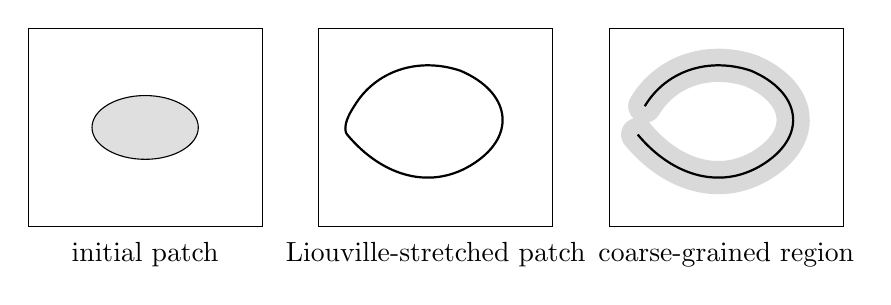
\begin{tikzpicture}[scale=0.9]
\draw (-0.5,-1.4) rectangle (2.8,1.4);
\fill[gray!25] (1.15,0) ellipse (0.75 and 0.45);
\draw (1.15,0) ellipse (0.75 and 0.45);
\node at (1.15,-1.8) {initial patch};

\draw (3.6,-1.4) rectangle (6.9,1.4);
\draw[line width=0.8pt]
(4.0,-0.1) .. controls (4.5,-0.7) and (5.2,-0.9) .. (5.8,-0.5)
.. controls (6.4,-0.1) and (6.3,0.5) .. (5.6,0.8)
.. controls (5.0,1.0) and (4.4,0.8) .. (4.1,0.3)
.. controls (3.9,0.0) and (4.0,-0.1) .. (4.0,-0.1);
\node at (5.25,-1.8) {Liouville-stretched patch};

\draw (7.7,-1.4) rectangle (11.0,1.4);
\draw[line width=12pt, gray!30, line cap=round]
(8.1,-0.1) .. controls (8.6,-0.7) and (9.3,-0.9) .. (9.9,-0.5)
.. controls (10.5,-0.1) and (10.4,0.5) .. (9.7,0.8)
.. controls (9.1,1.0) and (8.5,0.8) .. (8.2,0.3);
\draw[line width=0.8pt]
(8.1,-0.1) .. controls (8.6,-0.7) and (9.3,-0.9) .. (9.9,-0.5)
.. controls (10.5,-0.1) and (10.4,0.5) .. (9.7,0.8)
.. controls (9.1,1.0) and (8.5,0.8) .. (8.2,0.3);
\node at (9.35,-1.8) {coarse-grained region};
\end{tikzpicture}
\caption{The lecture's phase-space picture. A compact patch flows into a long thin ``snake'' of the same exact volume, while finite resolution replaces the fine structure by a larger effective occupied region.}
\end{figure}

\subsection{Question \& Answer}

\paragraph{Question.} If Liouville's theorem preserves the phase-space volume exactly, how can entropy increase at all?

\paragraph{Answer.} At the fully resolved microscopic level it does not. The entropy relevant to the second law is a coarse-grained entropy. Real experiments do not resolve arbitrarily nearby phase points. A patch that has been stretched into a thin filament therefore does not remain a thin filament in our description. It is replaced by finite-resolution blobs, and those blobs cover a larger region.

So the relevant entropy is
\begin{equation}
S_{\mathrm{cg}}\propto \log V_{\mathrm{coarse}},
\qquad
V_{\mathrm{coarse}}\ge V_{\mathrm{blob}}.
\end{equation}
The increase is not a violation of Liouville's theorem. It is the consequence of losing track of fine structure.

This is exactly the cotton analogy from the lecture. If one adds up the actual volumes of the fibers, the volume may remain nearly unchanged. But if one cannot resolve those fibers and sees only the fluffed-out cotton, the apparent occupied volume has increased. So too in phase space.

The lecture is very explicit on a deeper point here: entropy is not simply a property of the system by itself. It is a property of the system together with what we know, or can resolve, about the system.

\section{Chaos, Recurrence, and the Probabilistic Law}

Why does coarse-graining become unavoidable? Because the thin snake does not remain a single thin snake. In a chaotic system it develops finer and finer tendrils. Whatever the resolving power is, wait long enough and the dynamics will create structure below that scale. That is where the second law really enters the lecture.

The operational content of chaos is then discussed at length. Nearby trajectories stay close for a while and then separate, so long-time prediction demands ever more precise initial data. In modern shorthand one expresses this by a positive Lyapunov exponent:
\begin{equation}
\delta\Gamma(t)\sim e^{\lambda t}\,\delta\Gamma(0),
\qquad \lambda>0,
\end{equation}
where \(\delta\Gamma\) denotes a small separation in phase space. The lecture does not derive such a formula formally, but it repeatedly describes exactly this phenomenon and later identifies it by name when a student asks about the ``Lyapunov coefficient.''

\subsection{Question \& Answer}

\paragraph{Question.} What does ``chaotic'' mean here, and how is it different from an ordinary instability?

\paragraph{Answer.} In the lecture's operational sense, a chaotic system is one in which nearby trajectories follow each other only for a while and then separate so fast that predictability effectively breaks down. For a fixed time \(t\), there is some tolerance \(\epsilon\) in the initial conditions that permits prediction up to time \(t\); but as \(t\) grows, that required precision becomes more and more severe.

The harmonic oscillator is the clean counterexample. In phase space it just goes around in circles, and nearby phase points stay nearby forever. A true two-body inverse-square problem behaves similarly. But the three-body problem is generically chaotic, and the double pendulum is a standard lecture example of the same phenomenon. In a merely local instability, such as balancing at the top of a hill, one has a special unstable point. In a chaotic system, the instability is spread much more broadly through the accessible phase space.

Once the system is chaotic and the accessible region of phase space is bounded, another feature appears. The system can wander through a finite region only so many ways before coming close again to where it once was. The lecture makes this concrete with the billiard-table analogy and then with the air-in-the-corner-of-the-room example.

\begin{figure}[h]
\centering
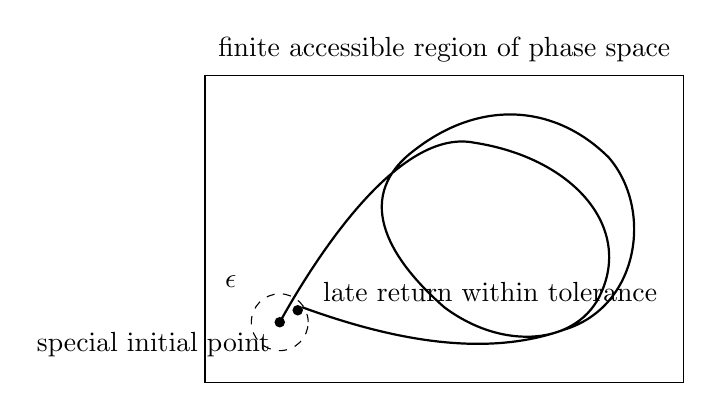
\begin{tikzpicture}[scale=0.95]
\draw (0,0) rectangle (6.4,4.1);
\node at (3.2,4.45) {finite accessible region of phase space};

\fill (1.0,0.8) circle (2pt);
\node[below left] at (1.0,0.8) {special initial point};

\draw[dashed] (1.0,0.8) circle (0.38);
\node[left] at (0.55,1.35) {\(\epsilon\)};

\draw[line width=0.8pt]
(1.0,0.8) .. controls (1.5,1.7) and (2.6,3.4) .. (3.6,3.2)
.. controls (4.9,3.0) and (5.7,2.1) .. (5.3,1.2)
.. controls (5.0,0.5) and (4.0,0.4) .. (3.2,1.0)
.. controls (2.4,1.7) and (2.0,2.5) .. (2.8,3.1)
.. controls (3.7,3.8) and (4.7,3.7) .. (5.4,3.0)
.. controls (6.0,2.3) and (5.8,1.0) .. (4.8,0.7)
.. controls (3.7,0.3) and (2.4,0.6) .. (1.3,1.0);

\fill (1.24,0.96) circle (2pt);
\node[right] at (1.45,1.2) {late return within tolerance};
\end{tikzpicture}
\caption{A schematic recurrence picture. The phase point wanders through a bounded accessible region and can return to an \(\epsilon\)-neighborhood of its starting point after a typically enormous time.}
\end{figure}

The right statement about recurrence is therefore not exact return to the same point with infinite precision. The right statement is return within some tolerance \(\epsilon\). For any fixed \(\epsilon\), the recurrence time is finite, though for a system with many degrees of freedom it may be unimaginably large. That is why the air in a room can spread to equilibrium and yet, in principle, return to something like its original very special configuration if one waits long enough.

So coarse-grained entropy increase does not abolish reversibility. The system can still return near the initial configuration. That is why the lecturer ends not with the slogan ``entropy always increases'' but with Boltzmann's more careful formulation: from any given configuration, the next configuration is overwhelmingly more likely to have larger entropy than smaller entropy. Entropy probably increases.

This is not a weakening of the second law. It is the real content of the law when one takes microscopic reversibility seriously.

\section{Summary}

The lecture unfolds in a very deliberate order. We begin by deferring the second law and first extracting something concrete from statistical mechanics: an estimate for the speed of sound in a dilute gas. We then move to the harmonic oscillator and derive the classical result
\begin{equation}
E=T,
\end{equation}
with equal kinetic and potential contributions \(T/2\). That result is both elegant and absurd for very stiff oscillators, and quantum mechanics resolves the absurdity by introducing the threshold
\begin{equation}
T\sim \hbar\omega.
\end{equation}
Above that threshold the oscillator behaves classically; below it, the mode is frozen out.

From there the lesson broadens naturally to molecules, solids, and strings: as temperature rises, more degrees of freedom are activated. Only after that preparation do we return to the second law. Liouville's theorem preserves the exact phase-space volume, but coarse-graining does not preserve the effective occupied volume of a filamented patch. Chaos ensures that the fine structure gets finer and finer, and recurrence reminds us that microscopic reversibility is never really gone. The resolution is therefore probabilistic. Entropy need not increase in every logically possible step, but in a system with many degrees of freedom it overwhelmingly tends to.